% Author: Grayson Orr
% Course: IN721: Mobile Application Development

\documentclass{article}
\author{}

\usepackage{graphicx}
\usepackage{wrapfig}
\usepackage{enumerate}
\usepackage{hyperref}
\usepackage[margin = 2.25cm]{geometry}
\usepackage[table]{xcolor}
\usepackage{fancyhdr}
\hypersetup{
  colorlinks = true,
  urlcolor = blue
}
\setlength\parindent{0pt}
\pagestyle{fancy}
\fancyhf{}
\rhead{College of Engineering, Construction and Living Sciences\\Bachelor of Information Technology}
\lfoot{Practical 03: Animal Sounds\\Version 1, Semester One, 2020}
\rfoot{\thepage}

\begin{document}

\begin{figure}
    \centering
    
\includegraphics[width=50mm]{./img/logo.png}
\end{figure}

\title{College of Engineering, Construction and Living Sciences\\Bachelor of Information Technology\\IN721: Mobile Application Development\\Level 7, Credits 15\\\textbf{Practical 03: Animal Sounds}}
\date{}
\maketitle

\section*{Assessment Overview}
In this assessment, you will refactor the provided application's code to use \textbf{LiveData}, \textbf{ViewModel} \& \textbf{Data Binding}. Also, you will research \& implement a splash screen \& \textbf{Fragment} animation using the provided resources. This assessment contributes \textbf{9\%} towards your final mark in \textbf{IN721: Mobile Application Development}.

\section*{Learning Outcomes}
At the successful completion of this course, learners will be able to: 
\begin{enumerate}
	\item Implement \& publish complete, non-trivial, industry-standard mobile applications following sound architectural \& code-quality standards.
	\item Identify relevant use cases for a mobile computing scenario \& incorporate them into an effective user experience design.
	\item Follow industry standard software engineering practice in the design of mobile applications.
\end{enumerate} 

\section*{Assessment Table}
\renewcommand{\arraystretch}{1.5}
\begin{tabular}{|l|l|l|l|l|}
	\hline      
	\vtop{\hbox{\strut \textbf{Assessment}}\hbox{\strut \textbf{Activity}}} & \textbf{Weighting} & \vtop{\hbox{\strut \textbf{Learning}}\hbox{\strut \textbf{Outcomes}}} & \vtop{\hbox{\strut \textbf{Assessment}}\hbox{\strut \textbf{Grading Scheme}}} & \vtop{\hbox{\strut \textbf{Completion}}\hbox{\strut \textbf{Requirements}}} \\
	                            
	\hline
	                                
	\small Practical                                          & \small 20\%        & \small 2, 3                                                         & \small CRA                                                                    & \small Cumulative                                                           \\ \hline  
	\small Project                                                             & \small 80\%        & \small 1, 2, 3                                                       & \small CRA                                                                    & \small Cumulative                                                           \\ \hline 
\end{tabular}

\section*{Conditions of Assessment}
You will complete this individual assessment inside \& outside timetabled class time. This assessment will need to be completed by \textbf{Friday, 9 April 2021} at \textbf{5:00 PM}. 

\section*{Pass Criteria}
This assessment is criterion-referenced (CRA) with a cumulative pass mark of \textbf{50\%} over all assessments in \textbf{IN721: Mobile Application Development}.

\section*{Authenticity}
All parts of your submitted assessment must be completely your work \& any references must be cited appropriately including, externally-sourced graphic elements. Provide your references in a \textbf{README.md} file. All media must be royalty free (or legally purchased) for educational use. Failure to do this will result in a mark of \textbf{zero} for this assessment.

\section*{Policy on Submissions, Extensions, Resubmissions \& Resits}
The school's process concerning submissions, extensions, resubmissions \& resits complies with \textbf{Otago Polytechnic} policies. Learners can view policies on the \textbf{Otago Polytechnic} website located at \href{https://www.op.ac.nz/about-us/governance-and-management/policies}{https://www.op.ac.nz/about-us/governance-and-management/policies}.

\section*{Submissions}
You must submit all program files via \textbf{GitHub Classroom}. Here is the URL to the repository you will use for your submission – \href{https://classroom.github.com/a/VJIq7Ae0}{https://classroom.github.com/a/VJIq7Ae0}. Create a new branch called  \textbf{03-animal-sounds} from the \textbf{main} branch by running the command - \textbf{git checkout -b 03-animal-sounds}. This branch will be your development branch for this assessment. Once you have completed this assessment, create a pull request \& assign the \textbf{GitHub} user \textbf{grayson-orr} to a reviewer. \textbf{Do not} merge your own pull request. Late submissions will incur a \textbf{10\% penalty per day}, rolling over at \textbf{5:00 PM}.

\section*{Extensions}
Familiarise yourself with the assessment due date. If you need an extension, contact the course lecturer before the due date. If you require more than a week's extension, a medical certificate or support letter from your manager may be needed.

\section*{Resubmissions}
Learners may be requested to resubmit an assessment following a rework of part/s of the original assessment. Resubmissions are to be completed within a negotiable short time frame \& usually must be completed within the timing of the course to which the assessment relates. Resubmissions will be available to learners who have made a genuine attempt at the first assessment opportunity \& achieved a \textbf{D grade (40-49\%)}. The maximum grade awarded for resubmission will be \textbf{C-}.

\section*{Resits}
Resits \& reassessments are not applicable in \textbf{IN721: Mobile Application Development}.

\section*{Instructions - Learning Outcomes 2, 3}
\subsection*{Task One (3\%):}
In the \textbf{code-resources} directory, you have been provided a directory called \textbf{03-animal-sounds}. Familiarise yourself with the code \& functionality. Use the code examples from the \textbf{08-live-data} teaching session to refactor the application's code so that it is using \textbf{LiveData} with \textbf{ViewModel}. \\

Run your application on either an \textbf{Android Emulator} or \textbf{connect device}. \\ 

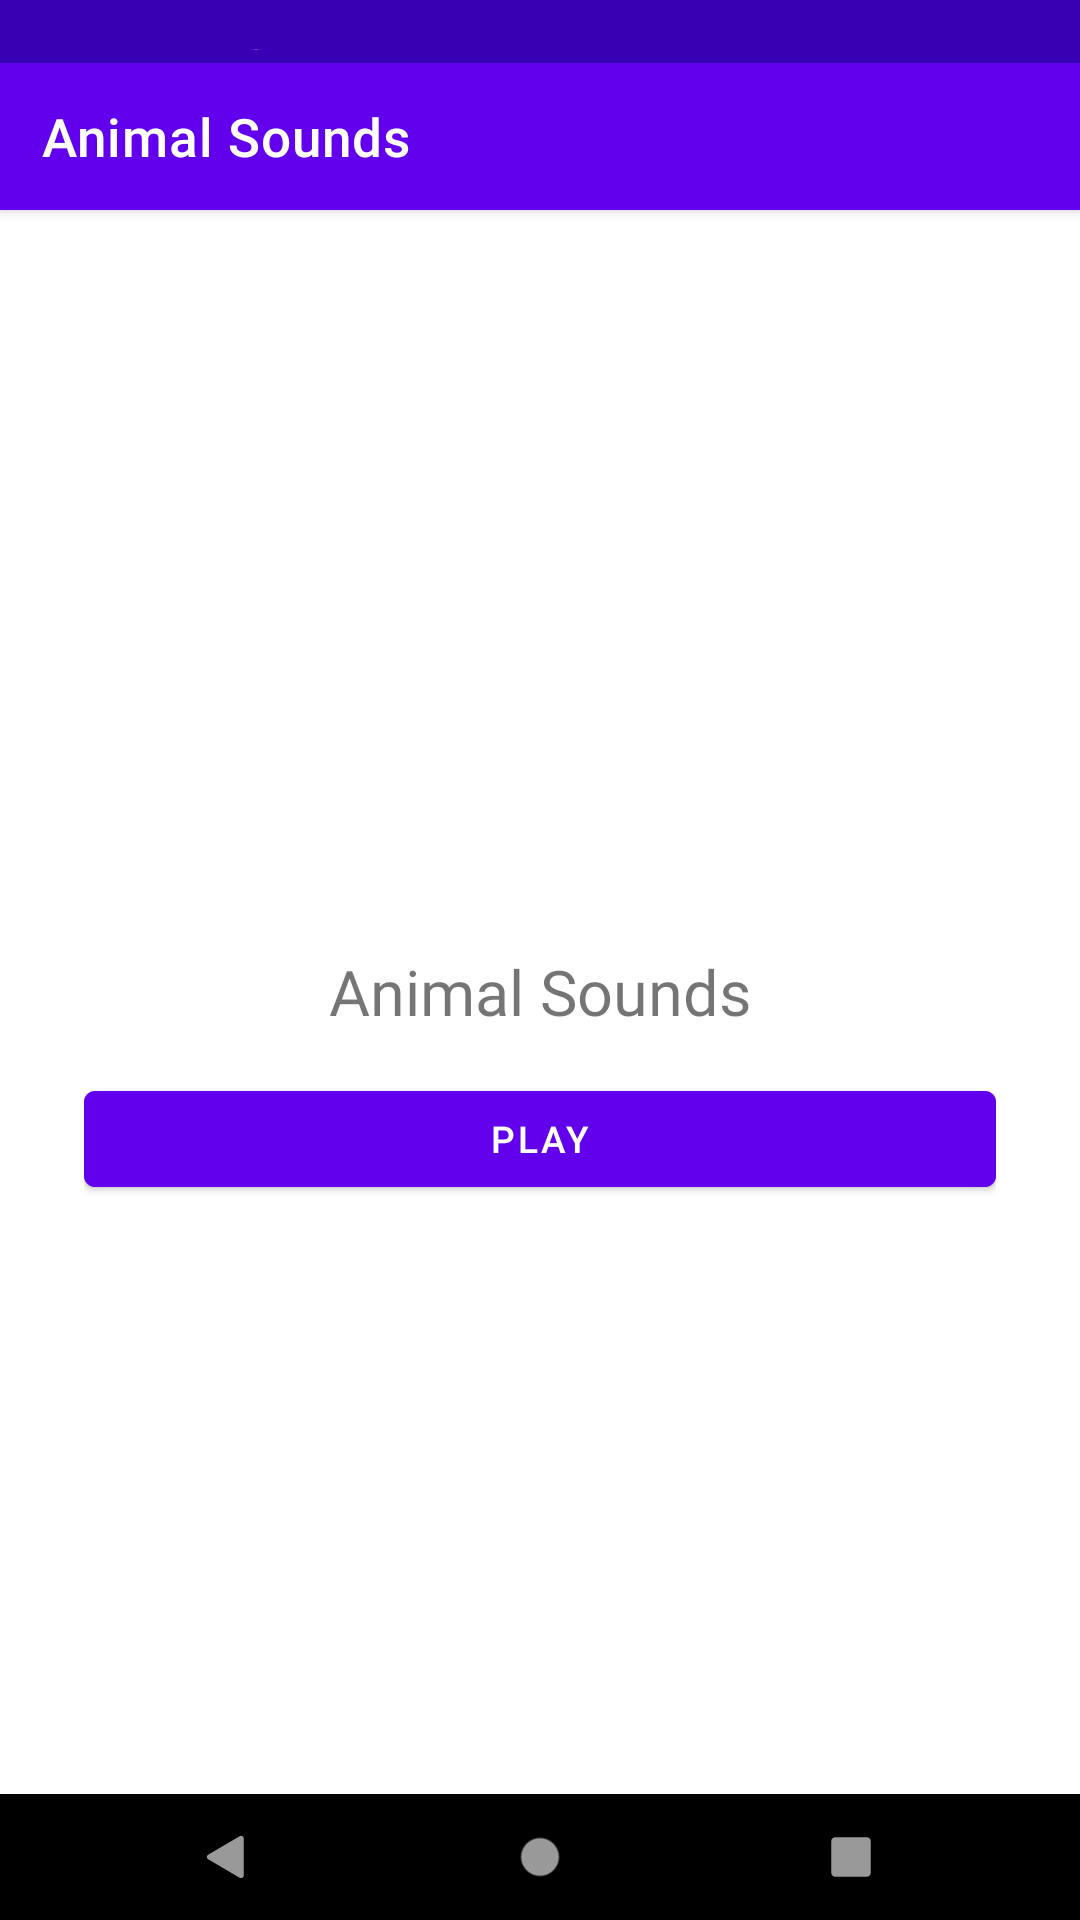
\includegraphics[width=5cm, height=9cm]{../tex/img/practicals/03-animal-sounds-1.png}
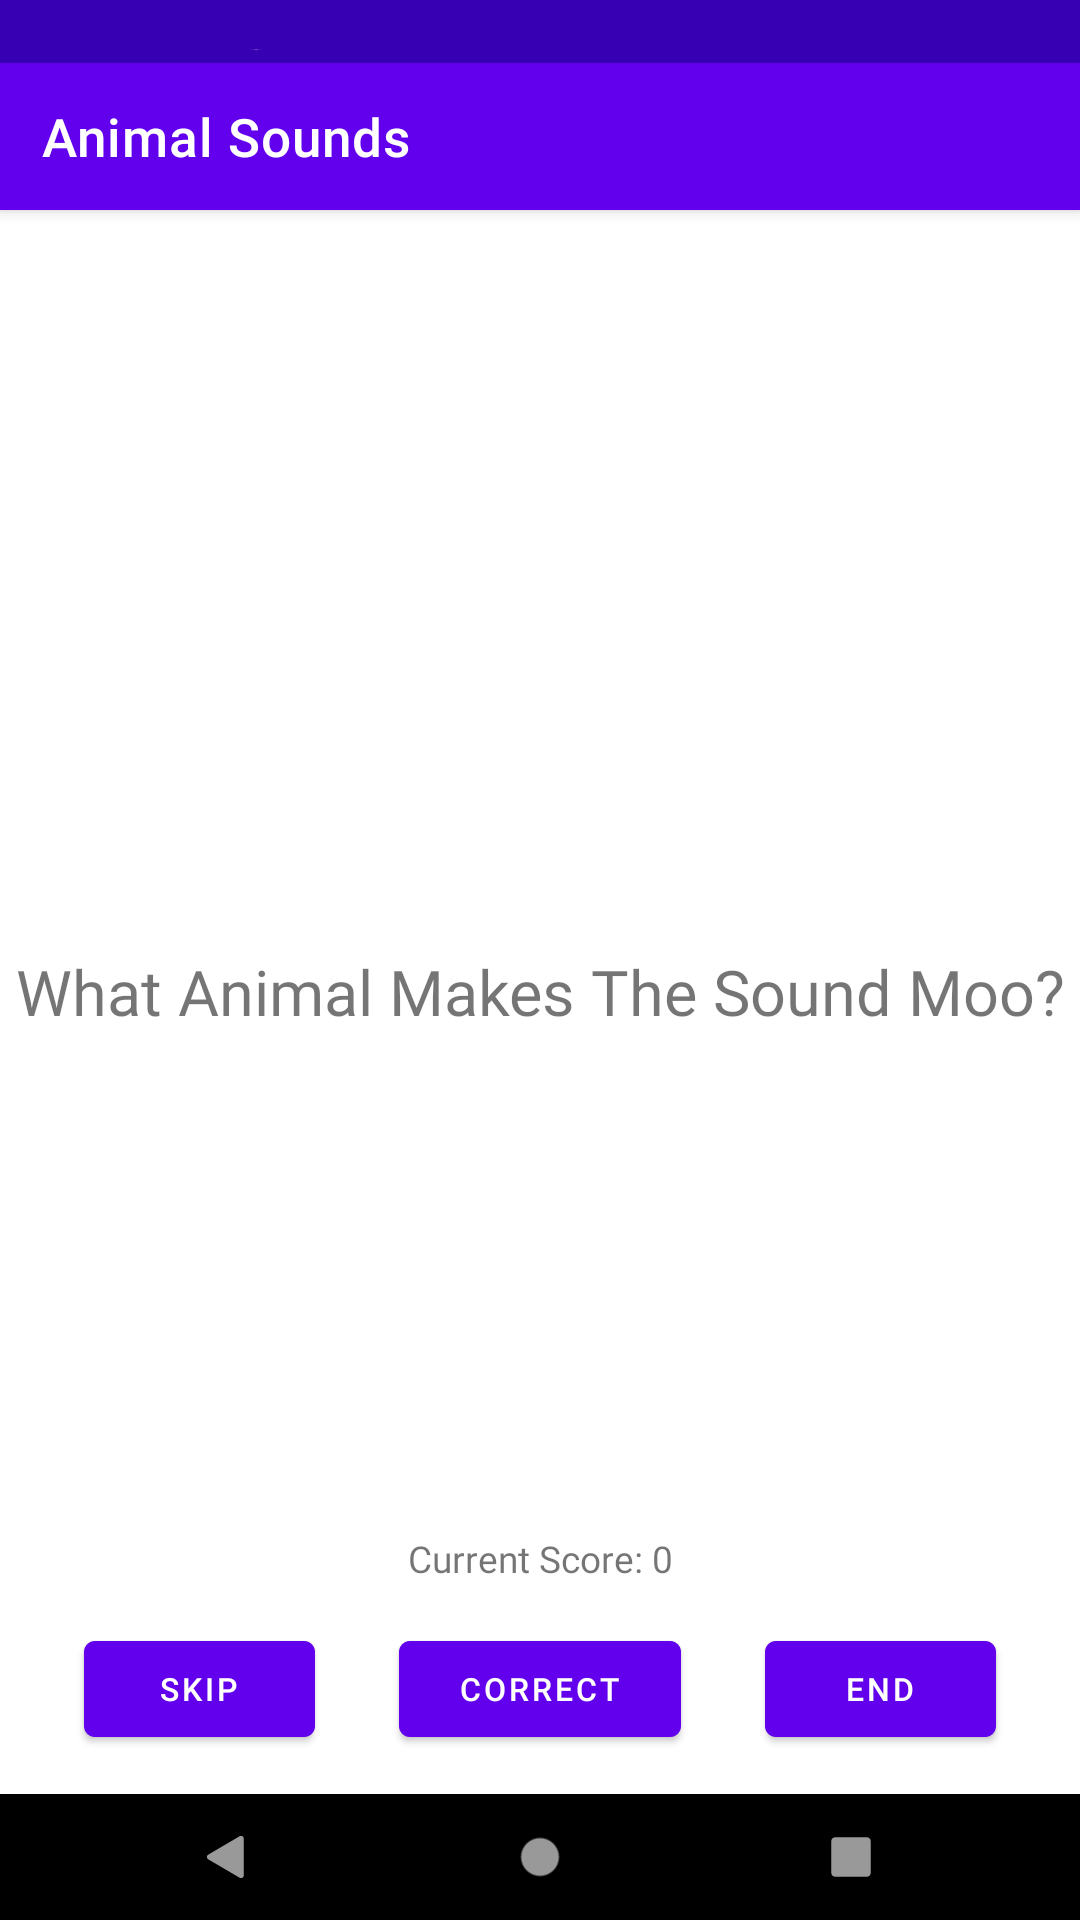
\includegraphics[width=5cm, height=9cm]{../tex/img/practicals/03-animal-sounds-2.png}
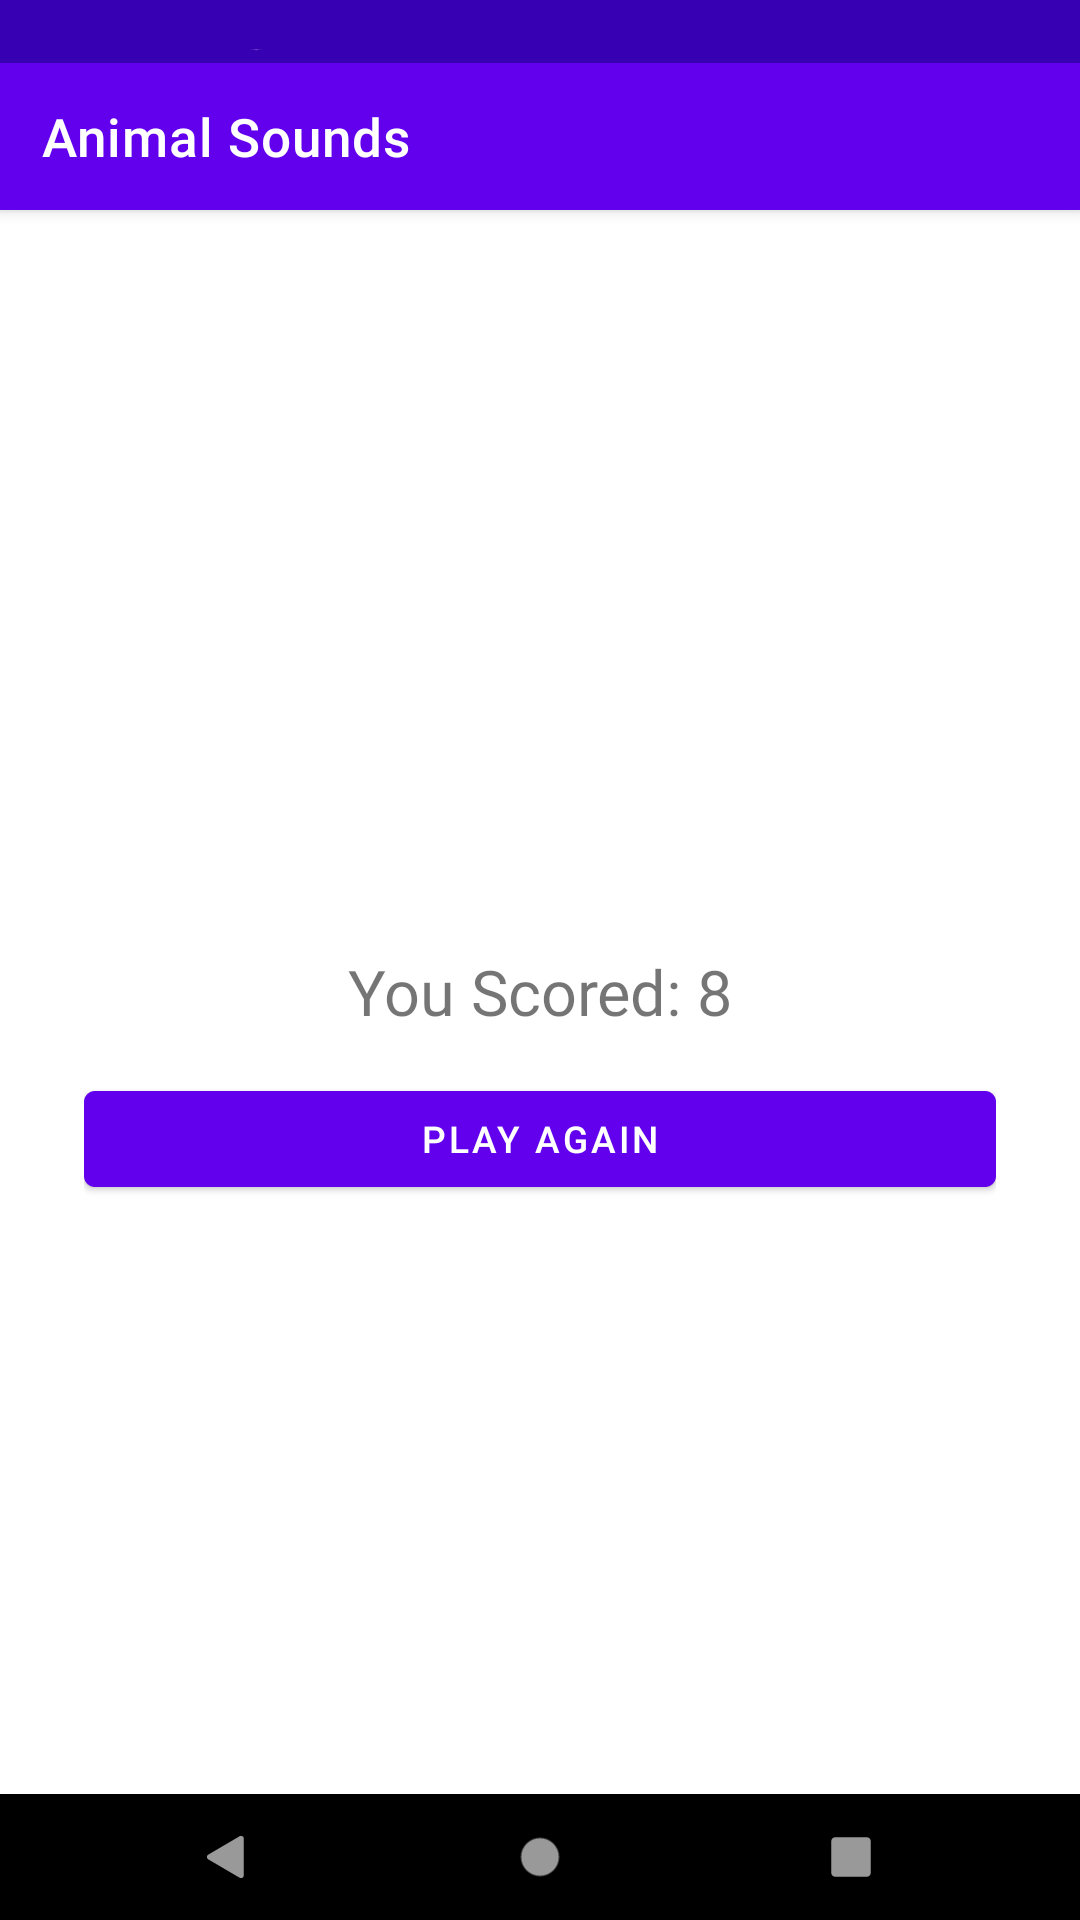
\includegraphics[width=5cm, height=9cm]{../tex/img/practicals/03-animal-sounds-3.png} \\

Commit your code to your repository for future reference.

\subsection*{Task Two (2\%):}
Create a new test file called \textbf{AnimalSoundsTest}. To do this, right-click on \textbf{op.mobile.app.dev.animal.sounds (androidTest) $>$ Kotlin Class/File}. In \textbf{AnimalSoundsTest.kt}, write five UI tests. To run your test file, right-click \textbf{AnimalSoundsTest.kt $>$ 'Run AnimalSoundsTest'}.

\subsection*{Task Three (2\%):}
Use the code examples from the \textbf{09-data-binding} teaching session to refactor the application's code so that it is using \textbf{Data Binding} with \textbf{LiveData} \& \textbf{ViewModel}. 

\subsection*{Task Four (1\%):}
Create a new activity file called \textbf{SplashScreenActivity}. Use the following resource to create an animated splash screen - \href{https://blog.mindorks.com/getting-started-with-lottie-animation-in-android}{https://blog.mindorks.com/getting-started-with-lottie-animation-in-android}. \textbf{Note:} this resource uses \textbf{MainActivity.kt} \& \textbf{activity\_main.xml}. Instead, use \textbf{SplashScreenActivity.kt} \& \textbf{activity\_splash\_screen.xml}. Remember, \textbf{MainActivity} is responsible for hosting the \textbf{Fragment} classes. In \textbf{AndroidManifest.xml}, change the launcher activity to \textbf{SplashScreenActivity}. Override the \textbf{theme} attribute \& set it to the value so that the \textbf{action bar} is hidden. 

\subsection*{Task Five (1\%):}
Create a new resource directory called \textbf{anim}. To do this, right-click on \textbf{res $>$ Android Resource Directory}. In the \textbf{New Resource Directory} window, change the \textbf{Directory name} \& \textbf{Resource type} to \textbf{anim}. Copy the four \textbf{XML} files in the \textbf{11-animations} directory to the \textbf{anim} directory. In \textbf{res/navigation/mobile\_navigation.xml}, declare an animation for sliding in \& out of a \textbf{Fragment}. If you are confused, please refer to the \textbf{11-animation} teaching session video.

\end{document}